\section{Evaluation}
\subsection{Prüfung der Anforderungen}\label{btc_evaluation}%Anforderungserfüllung}

Dieser Abschnitt behandelt in wie weit das beschriebene Konzept die in \ref{anforderungen} aufgelisteten Anforderungen erfüllt. Die jeweilige Anforderung wird zunächst wiederholt und anschließend genauer untersucht.

\subsubsection{1) Transparente Einzahlungen}
\textit{Die Einzahlung jedes Endnutzers ist für jeden anderen Endnutzer nachprüfbar.}\\\\
Diese Anforderung ist erfüllt, da jede Transaktion in der lokalen Datenbank jedes Peet-to-Peer Netzwerkteilnehmers aufgezeichnet wird. 
Auf der Webseite \cite{blockchain_info} kann man die Bitcoin Blockchain mithilfe eines sogenannten Blockchain-Explorers durchsuchen. Mit diesem Werkzeug kann man die Blöcke und die darin enthaltenen Transaktionen untersuchen. Nutzt man den Explorer einer Drittpartei, muss man darauf vertrauen, dass dieser auch den ''wahren'' Status der Blockchain anzeigt. Um dieses Risiko zu vermeiden kann jeder Teilnehmer mithilfe eines eigenen Bitcoin Full Nodes am Netzwerk teilnehmen. Dieser speichert die gesamte Blockchain und prüft alle Transaktionen und Blöcke gegen die Konsensregeln.\\
Der Bitcoin Full Node stellt eine API bereit, über die man den aktuellen Status der Blockchain abfragen kann. Der Befehl \textit{getblockchaininfo} liefert den aktuellen Zustand der Blockchain zurück. Dieser beinhaltet die Blocknummer des neusten Blocks und dessen Blockhash. Der Befehl \textit{gettransaction} gefolgt von der Transaktions-ID liefert Details über diese Transaktion. Die Webseite \cite{btc_api} dokumentiert diese Schnittstelle detailliert. 

\subsubsection{2) Gewinnerauswahl durch Zufallsfaktor}
\textit{Die Auswahl des Gewinners ist von einem zufälligen Faktor abhängig, auf den weder die Anwendung noch die Endnutzer einen Einfluss haben.}\\\\
Diese Anforderung wird nur bedingt erfüllt, da ein Teilnehmer des Peer-to-Peer Netzwerks sowohl ein Spieler als auch ein Miner sein kann. Ist dies der Fall besteht die Möglichkeit, dass der Miner einen validen Blockhash verwirft, sobald er merkt, dass er durch diesen Blockhash nicht zum Gewinner des Geldtopfes wird. Verwirft der Teilnehmer einen Blockhash, riskiert er den dadurch ausgeschütteten Blockreward. Ein solcher Angriff ist für einen Miner nur rentabel, falls die Spieleinsätze des Geldtopfes den Blockreward um ein vielfaches übersteigen.
Betrachten wir dazu das Bitcoin Netzwerk Anfang Februar 2018. Der Preis pro Bitcoin beträgt 8000 Euro. Der Mining Reward liegt bei 12,5 Bitcoin pro Block\footnote{Dieses Beispiel vernachlässigt die durch das Minen des Blocks erhaltenen Transaktionsgebühren.}. Für das Lösen eines gültigen Blocks erhält ein Miner somit 100000 Euro. Angenommen ein Miner besitzt 20 Prozent der Hashrate des gesamten Bitcoin-Netzwerks und nimmt an einem Topf mit 2 Personen teil. Dies bedeutet, dass sowohl der Miner als auch der andere Teilnehmer eine Gewinnwahrscheinlichkeit von 0,5 für einen zufälligen Blockhash haben.
Mit einer Wahrscheinlichkeit von 0,8 findet ein anderer Miner des Bitcoin Netzwerks und der Miner kann den Ausgang des Spiels nicht beeinflussen. Mit einer Wahrscheinlichkeit von 0,2 findet der Miner den Block und kann entscheiden, ob er den Block veröffentlicht oder verwirft. Entscheidet er sich den Block zu verwerfen, muss er einen weiteren Block vor dem Rest des Netzwerkes finden, um den Ausgang des Spiels beeinflussen zu können. Ab diesem Moment hat er wieder eine Wahrscheinlichkeit von 0,2, da es sich beim Mining um einen gedächtnislosen Prozess handelt. Die Wahrscheinlichkeit, dass der Miner einen zweiten gültigen Block findet ist daher sehr gering und liegt bei $0,2 * 0,2 = 0,04$. Auch dieser zweite gültige Block führt nur in 50 Prozent der Fälle zu einem Gewinn des Topfes.
\todo{Erwartungswert berechnen.}
%Die Berechnung des Erwartungswerts gibt eine Aussage ab welchem Einsatz es sich für den Miner lohnt einen gültigen Block zu verwerfen um den Ausgang des Spiels zu manipulieren. Sei $E$ der Einsatz des Topfes. 

%Da der Miner eine Hashrate von 20 Prozent hat, liegt die Wahrscheinlichkeit das der Miner den nächsten Block findet bei 0,2. Falls er den gefundene Blockhash verwirft, da er durch diesen seinen Glücksspieleinsatz verlieren würde, muss er es schaffen vor einem anderen Miner einen weiteren Blockhash zu berechnen. Ansonsten verliert er den Blockreward. Die Wahrscheinlichkeit das der Miner zwei gültige Blockhashs hintereinander findet, liegt bei 0,2 * 0,2 = 0,04 und ist somit verschwindend gering.

\subsubsection{3) Nachprüfbarkeit des Zufallsfaktor}
\textit{Jeder Endnutzer kann die Echtheit des zufälligen Faktors eigenständig nachprüfen.}\\\\
Da das Verfahren der Gewinnerauswahl im Vorhinein festgelegt ist und die Reihenfolge der Einzahlungstransaktionen in der Blockchain festgeschrieben steht, kann jeder Teilnehmer die Berechnung des Gewinners eigenständig nachvollziehen. Der Blockhash, der die Grundlage für die Gewinnerauswahl liefert, kann durch die Verwendung eines Bockchain-Explorers oder eines Full Nodes nachgeprüft werden. 
\subsubsection{4) Transparente Auszahlungen}
\textit{Die Auszahlung an den Gewinner muss transparent und somit für jeden Endnutzer nachprüfbar sein.}\\\\
Genau wie die Einzahlungen ist auch die Auszahlung für jeden Spieler mithilfe eines Blockchain-Explorers oder eines Bitcoin Full Nodes möglich. Jeder Teilnehmer kann somit für alle bereits abgeschlossenen Spiele nachprüfen, ob die Anwendung sich korrekt verhalten und eine Auszahlung getätigt hat. 
\subsubsection{5) Fairheit des Spiels}
\textit{Jeder Endnutzer besitzt die gleiche Gewinnwahrscheinlichkeit und niemand wird benachteiligt}.\\\\
Die Zuordnung der Spieler auf die Gewinnzahlen ist durch die Reihenfolge der Transaktionen in der Blockchain festgeschrieben. Eine nachträgliche Veränderung dieser Reihenfolge ist weder durch die Nutzer, noch durch die Glücksspielanwendung möglich.\footnote{Eine Veränderung der Reihenfolge ist nur durch einen sogenannten Blockchain-Fork möglich. (siehe Abschnitt \ref{sssec:btc_fork})}

Damit keiner der Spieler einen Vorteil hat, muss jeder Topf-Platz die gleiche Gewinnwahrscheinlichkeit haben.
Dies ist gegeben, falls jeder Teilnehmer die gleiche Anzahl Gewinnzahlen zugeordnet bekommt und falls das Auftreten jeder Gewinnzahl die gleiche Wahrscheinlichkeit besitzt. Durch die Einschränkung der Topfgröße auf 2, 5 und 10 Teilnehmer bekommt jeder Spieler durch die Modulo-Funktion genau gleich viele Gewinnzahlen zugeordnet. Die Monte-Carlo-Simulation aus Abschnitt \ref{btc_distribution} legt nahe, dass die letzte Dezimalziffer der Werte der von Bitcoin verwendeten SHA-256 Hashfunktion gleichverteilt sind. Somit ist das Auftreten jeder Gewinnzahl gleich wahrscheinlich und die Anforderung erfüllt.

\subsection{Gewinnerauswahl}\label{btc_gewinnerauswahl}
Die Gewinnerauswahl kann entweder durch den gesamten Blockhash-Wert oder auf Basis der letzten Blockziffer vorgenommen werden.
Beide Methoden haben Vor- und Nachteile. Variante eins erlaubt beliebige Topfgrößen, ist dafür aber schwieriger für den Endnutzer zu verifizieren. Die Verifizierung erfordert eine Modulo-Rechnung mit einer sehr großen Zahl. Variante zwei ist dagegen leicht zu verifizieren, erlaubt allerdings nur die Topfgrößen zwei, fünf und zehn. Bei der Topfgröße von zwei sind beiden Spielern fünf Gewinnzahlen zugeordnet. Bei der Topfgröße von fünf besitzt jeder Teilnehmer genau 2 Gewinnzahlen. Bei einer Topfgröße von zehn wird jedem Teilnehmer genau eine Gewinnzahl zugeordnet. 
Nimmt man hingegen eine Topfgröße von 3,4,6,7,8 und 9 führt dies dazu das manche Teilnehmer eine signifikant höhere Gewinnchance haben.
Bei der Topfgröße von 3 sind die Gewinnzahlen durch die Modulo-Funktion folgendermaßen verteilt:
\begin{itemize}
\item Spieler 1 hat die Gewinnzahlen 0, 3, 6 und 9.
\item Spieler 2 hat die Gewinnzahlen 1, 4 und 7.
\item Spieler 3 hat die Gewinnzahlen 2, 5 und 8.
\end{itemize}
Somit hat Spieler 1 eine Gewinnwahrscheinlichkeit von $\frac{4}{10}$, Spieler 2 und 3 hingegen nur eine Gewinnwahrscheinlichkeit von $\frac{3}{10}$. Es kommt also vor, dass eine Teilmenge der Spieler genau eine Gewinnzahl mehr als der Rest der Teilnehmer hat.

Nimmt man den gesamten Blockhash zur Gewinnerauswahl ist die dadurch entstehende Ungerechtigkeit verschwindend gering und kann vernachlässigt werden. Dies ist der Fall, da die aus dem Blockhash resultierende Dezimalzahl in der Praxis sehr groß ist und jeder Spieler somit mehrere Millionen von Gewinnzahlen hat.

\subsection{Verteilung der Blockhash-Werte}\label{btc_distribution}
Der Blockhash eines Blocks wird durch die verwendete kryptographische Hashfunktion der Kryptowährung festgelegt. Die Verteilung der Werte wird somit von der verwendeten kryptographische Hashfunktion festgelegt.\\
Eine kryptografische Hashfunktion ist eine stark kollisionsresistente Einweg-Hashfunktion.\\
Eine Hashfunktion h heißt
\begin{itemize}
\item \textit{Einwegfunktion} genau dann, wenn es schwierig ist, zu gegebenem $_{Y0}$ ein $_{X0}$ zu finden mit $h(x_{0}) = y_{0}$.
\item \textit{schwach kollisionsresistent} genau dann, wenn es schwierig ist, zu einem gegebenen $x$ ein $x' \neq x$ zu finden mit $h(x) = h(x')$.
\item \emph{stark kollisionsresistent} genau dann, wenn es schwierig ist, $x$ und $x'$ zu finden
mit $x \neq x'$ und $h(x) = h(x')$.
\end{itemize}Die Eigenschaften der starken Kollisionsresistenz und der Einwegfunktion sagen nichts über die Verteilung der resultierenden Werte aus. Bei der Auswahl der Kryptowährung muss also gesondert auf die Verteilung der verwendete Hashfunktion geachtet werden. Sollte die verwendete kryptographische Hashfunktion keine Gleichverteilung liefern, kann der Blockhash dennoch den nötigen Zufall liefern indem dieser mit einer geeigneten Hashfunktion erneut gehasht wird.\\\\
Bitcoin verwendet die kryptographische Hashfunktion SHA256.
Die folgende Monte-Carlo-Simulation legt nahe, dass die Resultate der SHA256 gleichverteilt sind.
\begin{verbatim}
h=SHA256 n=1000000
for i 1 -> n
    hash = h(i);
    result[lastDigit(hash)]++
\end{verbatim}
\begin{minipage}{0.5\textwidth}
\begin{verbatim}
Ausgabe:
result[0] =  99765
result[1] = 100488
result[2] =  99913
result[3] = 100745
result[4] = 100272
result[5] =  99649
result[6] =  99430
result[7] =  99788
result[8] =  99666
result[9] = 100284
\end{verbatim}
\end{minipage}
\begin{minipage}{0.5\textwidth}
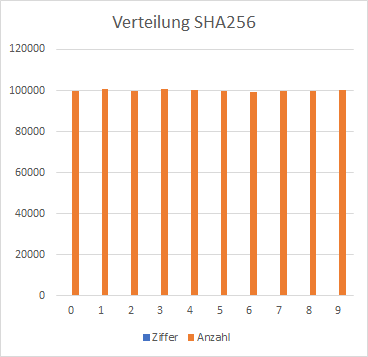
\includegraphics[width=\textwidth]{Figures/verteilung_sha256}
\centering
\decoRule
\captionof{figure}{Verteilung der SHA256 Hashfunktion}
\label{fig:verteilung_sha256}
\end{minipage}

\subsection{Auszahlungstransaktion} \label{sssec:Auszahlungstransaktion}
Die Glücksspielanwendung erzeugt für jede Einzahlung eine eigene Einzahlungsadresse statt für jeden Benutzer die gleiche Adresse zu verwenden. Dies hat den Vorteil, dass die Anwendung dem Benutzer anzeigen kann, dass seine Bitcoin Einzahlung eingegangen ist. Die folgenden Abbildungen betrachten die Auszahlungstransaktion des Beispiels aus Abschnitt \ref{ssec:btc_gui} betrachtet.

\begin{figure}[H]
\centering
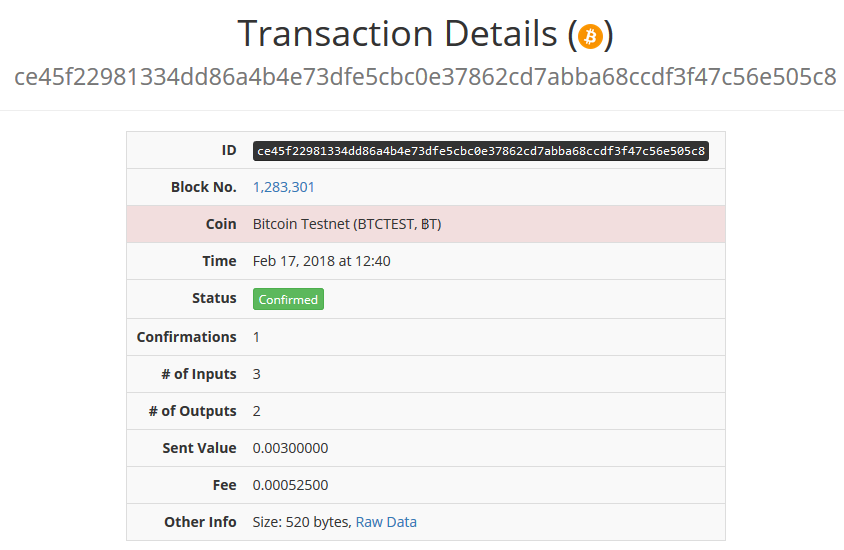
\includegraphics[width=1\linewidth]{Figures/btc_gui/btc_txn}
\decoRule
\caption{Auszahlungstransaktion Details}
\label{fig:btc_txn}
\end{figure}

Abbildung \ref{fig:btc_txn} zeigt in welchen Block die Transaktion aufgenommen wurde, den Status, den Wert, die Transaktionsgebühr und die Größe der Transaktion.
\footnote{Momentan zahlt die Glücksspielanwendung die Auszahlungstransaktionsgebühr aus eigener Tasche. Eigentlich müsste die Transaktionsgebühr von dem Gewinnbetrag abgezogen werden.}

\begin{figure}[H]
\centering
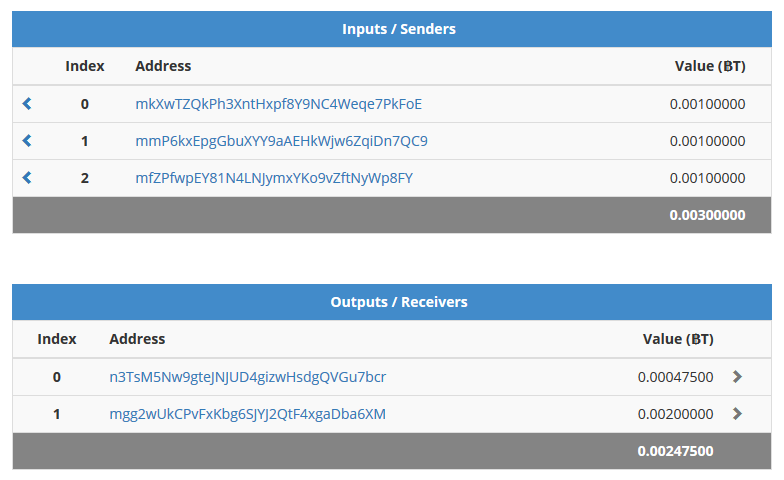
\includegraphics[width=1\linewidth]{Figures/btc_gui/btc_txn_input_output}
\decoRule
\caption{Auszahlungstransaktion Inputs und Outputs}
\label{fig:btc_txn_input_output}
\end{figure}


Abbildung \ref{fig:btc_txn_input_output} zeigt welche Inputs und Outputs für die Transaktion verwendet wurden. Output Adresse 1 gehört der Wallet der Glücksspielanwendung und stellt die Wechselgeldadresse dar.


\begin{figure}[H]
\centering
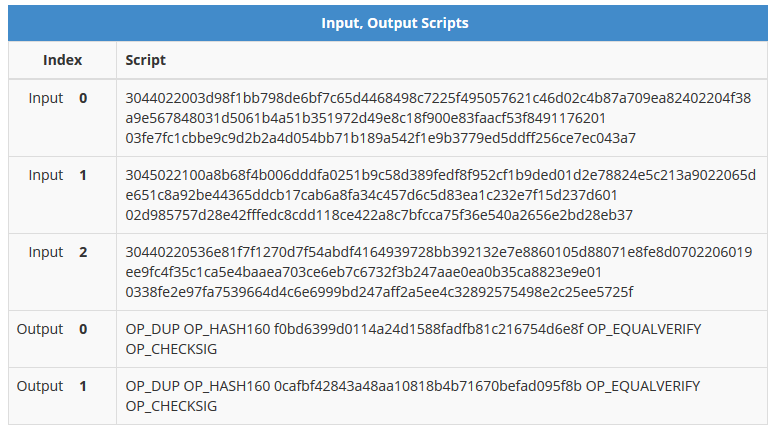
\includegraphics[width=1\linewidth]{Figures/btc_gui/btc_txn_input_output_scripts}
\decoRule
\caption{Auszahlungstransaktion Skripts}
\label{fig:btc_txn_input_output_scripts}
\end{figure}

Die Anwendung muss in der Auszahlungstransaktion für jede Input Adresse eine gültige Signatur angeben, obwohl alle Adressen von der gleichen Wallet kontrolliert werden. Hier könnte in Zukunft die Verwendung sogenannter Schnorr Multi-Signaturen \cite{schnorr_sig} aushelfen. Durch diese lassen sich alle Signaturen der Inputs durch eine einzige Signatur ersetzen.

\subsection{Blockchain Mining Varianz}
Der Begriff Blockchain Mining Varianz beschreibt den Umstand, dass die Miner des Netzwerkes entweder Glück oder Pech bei der Suche nach dem nächsten gültigen Blockhash haben können. Bei Bitcoin gibt es daher nicht genau alle 10 Minuten einen neuen Block, sonder durchschnittlich alle 10 Minuten. Für die Glücksspielanwendung bedeutet dies, dass die Zeit zwischen der letzten Einzahlung und der Auswahl des Gewinners variieren kann. In der Praxis kommt es vor, dass man 30 Minuten und mehr auf den nächsten Block warten muss. Dies ist für den Spieler eine recht lange Zeit. Das Proposal \cite{bobtail} liefert ein Verfahren, das die Blockchain Mining Varianz stark verringert. Dieser Vorschlag ist bisher allerdings noch nicht in den Bitcoin Sourcecode eingeflossen.
Eine andere Möglichkeit die Wartezeit für den Spieler zu verringern ist es eine  Kryptowährung mit einer geringeren Blockzeit zu verwenden. Beispiele hierfür sind LiteCoin mit einer Blockzeit von 2,5 Minuten, die auf Privatsphäre spezialisierte Währung Monero mit einer Blockzeit von 2 Minuten und Ethereum mit einer Blockzeit von 12 Sekunden. Bei einer geringen Blockzeit kommt es häufiger zu sogenannten Blockchain Forks. Weitere Informationen zu den genannten Kryptowährungen sind unter \cite{coin_ltc}, \cite{coin_xmr} und \cite{coin_eth} verfügbar.

\subsection{Blockchain Forks} \label{sssec:btc_fork}
Blockchain Forks entstehen, falls zwei Miner unabhängig voneinander mehr oder weniger gleichzeitig einen validen Block finden. Beide Miner broadcasten ihren Block schnellstmöglich an die Teilnehmer des Peer-to-Peer Netzwerks. Aufgrund von Netzwerkverzögerungen kommt es nun dazu, dass ein Teil des Netzwerks Block 1 und der restliche Teil des Netzwerks Block 2 zuerst enthält. Beide Blockchain-Ketten sind nun gleich lang.
\begin{figure}[H]
\centering
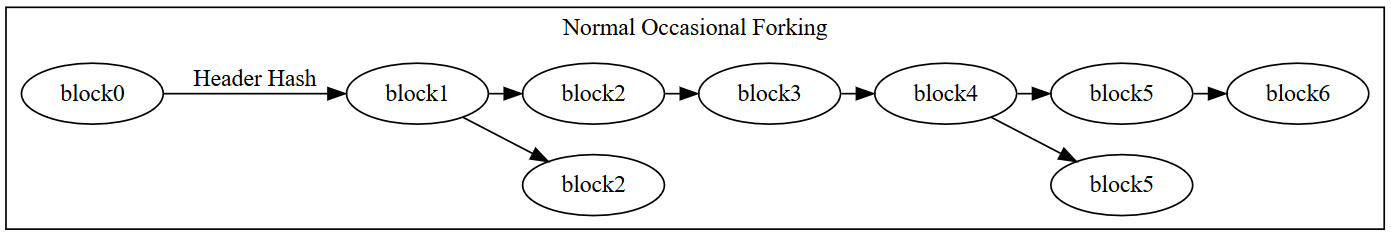
\includegraphics[width=1\linewidth]{Figures/btc/fork_normal}
\decoRule
\caption{Bitcoin Fork}
\label{fig:fork_normal}
\end{figure}
Der nächste gefundene Block entscheidet, auf welche Kette sich das Netzwerk einigt\footnote{Unter der Annahme, dass es nicht erneut zu einem Blockchain Fork kommt.}. Die Bitcoin Konsensregeln legen fest, dass die Teilnehmer des Netzwerks immer der längsten Kette, die somit am meisten Proof-of-Work beinhaltet, folgen. Dies erlaubt es jedem Bitcoin Knoten, ohne Trusted Third Party festzustellen, welche Version der Blockchain die echte ist. Forks kommen bei Bitcoin durch die hohe Hashrate des Netzwerks und die somit sehr hohe Difficulty recht selten vor. \cite{orphaned-blocks} zeigt an, wie oft gültige Blöcke gefunden und nicht Teil der längsten Blockchain werden.

\subsection{Betrugsmöglichkeiten}

Dieser Abschnitt betrachtet in wie weit die Glücksspielanwendung potentielle Spieler betrügen kann, sollte sie gehackt und zu ausschließlich diesem Zweck modifiziert werden.
Die Anwendung hat die volle Kontrolle darüber welche Ausgabe sie dem Benutzer anzeigt. Sie hat allerdings keine Kontrolle über den Status der Blockchain. 

Die Anwendung könnte beispielsweise anzeigen, dass der Topf nach der Einzahlung durch einen Spieler immer noch leer ist. Die Transaktion auf die Einzahlungsadresse existiert dann zwar in der Blockchain allerdings reagiert die Anwendung nicht entsprechend. Dies hat zur Folge, dass jeder Spieler der eine Einzahlung tätigt, sein Geld verliert. Allerdings merkt der Benutzer dies und kann somit eine weitere Verwendung der Anwendung unterlassen. Ein solch plumper Manipulationsversuch fällt somit direkt auf.

Ein weitere Betrugsmöglichkeit ist, dass die Glücksspielanwendung sich bis zur Gewinnerauswahl korrekt verhält, dann allerdings keine Auszahlung tätigt. Alle einzahlenden Spieler merken den Betrug, verlieren aber dennoch ihr Geld.

Bei beiden vorgestellten Betrugsversuchen fällt der Betrug immer mindestens einem Spieler auf. Die Verwendung einer solchen Anwendung macht nur Sinn, falls man den Betreiber des Services kennt und diesen im Zweifel juristisch haftbar machen kann.\\
Das folgende Kapitel betrachtet wie sogenannte Smart Contracts dieses Problem lösen. Ein Smart Contract erlauben es die Geschäftslogik der Glücksspielanwendung in die Blockchain zu schreiben. Die Geschäftslogik wird somit nicht mehr von der Anwendung, sondern von jedem Teilnehmer des Peer-to-Peer Netzwerks ausgeführt.